\documentclass[11pt, oneside]{article} 
\usepackage{geometry}
\geometry{letterpaper} 
\usepackage{graphicx}
	
\usepackage{amssymb}
\usepackage{amsmath}
\usepackage{parskip}
\usepackage{color}
\usepackage{hyperref}

\graphicspath{{/Users/telliott_admin/Dropbox/Tex/png/}}
% \begin{center} 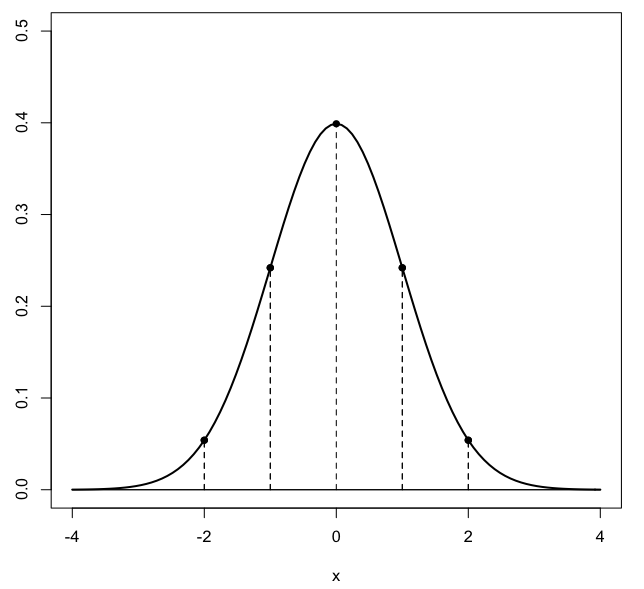
\includegraphics [scale=0.4] {gauss3.png} \end{center}

%break
\title{Numerical introduction}
\date{}

\begin{document}
\maketitle
\Large
It has been shown that some important integrals cannot be "solved" analytically (i.e.  we cannot find $F(x)$).  For example, the normal distribution (with mean and standard deviation both equal to $1$) is described by this probability density function:

\[ f(x) = \frac{1}{\sqrt{2 \pi}} \ e^{-x^2/2} \]

To find the expected value or probability that the value lies between bounds $a$ and $b$ we should compute:

\[  \int_a^b f(x) \ dx \]

However, there is no function $F(x)$ such that $F'(x) = f(x)$, so we cannot solve the equation in the normal way by computing $F(b) - F(a)$.

To compute the integral, we fall back on Riemann sums.  Divide the closed range $[a,b]$ into $N$ rectangles whose individual height is the value $f(x)$ somewhere in the rectangle, and then compute the sum of $\Delta x \times f(x)$ over the whole interval.  A simple approach uses rectangles of constant width (equal to $b-a/N$).

Using Python:

\url{https://gist.github.com/telliott99/5a1190217a130c7ee01dee17ea483f7b}

I hope the flow is clear.  The function $\tt{get\_xvalues}$ generates a list of $x$-values starting from the middle of the first step past $a$ and continuing to the last step just before $b$.  $\tt{integrate}$ simply computes $f(x)$ for each $x$-value, sums all of those values, and adjusts for the width of the steps (rectangles).

We integrate $f(x) = x^2$ over the ranges $[0,1]$ and $[1,2]$ and obtain the expected results ($1/3$ and $7/3$).

We also integrate the normal probability density function over ranges $[-2,2]$ to $[-10,10]$.  With standard deviation equal to $1$, we obtain the expected result that $95 \%$ of the density lies within two standard deviations of the mean.  Essentially all of the density lies within four standard deviations of the mean.

And finding that the total area equals $1$ confirms that the normalization factor $1/\sqrt{2 \pi}$ is correct.  That is, the value of the unnormalized integral is equal to $\sqrt{2 \pi}$.

\subsection*{Refinements}
Classically, the major improvement to be made to this algorithm is to make a more accurate estimation of the area for each small rectangle.  This is not so important with fast computers.  For example, with a million steps rather than 100, I obtain 

\begin{verbatim}
    > python numerical_int.py 
    0.333333333333
    2.33333333333
    >
\end{verbatim}

for the first two integrations, in about two seconds.

The calculation above uses the midpoint rule, where $f(x)$ is evaluated at the midpoint of the range.

\begin{center} 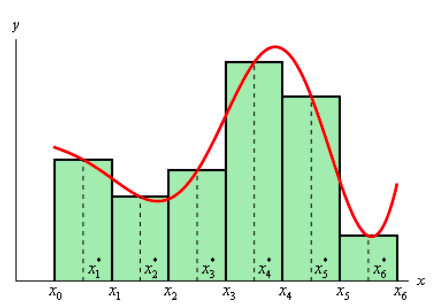
\includegraphics [scale=0.4] {midpoint_rule.png} \end{center}

The step size is computed and used to generate a list of values where each rectangle starts, then half the step is added to give the midpoint.  

If we think of $a$ and $b$ as the bounds for each small rectangle, then the average of $a$ and $b$ is the midpoint:
\[ m = \frac{a+b}{2} \]

We evaluate $f(m)$, the function at the midpoint, and then multiply by the width:
\[ M = f(m) \cdot (b-a) \]

Simpson's rule is a more sophisticated approach that uses:
\[ \frac{f(a) + 4f(m) + f(b) }{6} \cdot (b-a) \]

\begin{center} 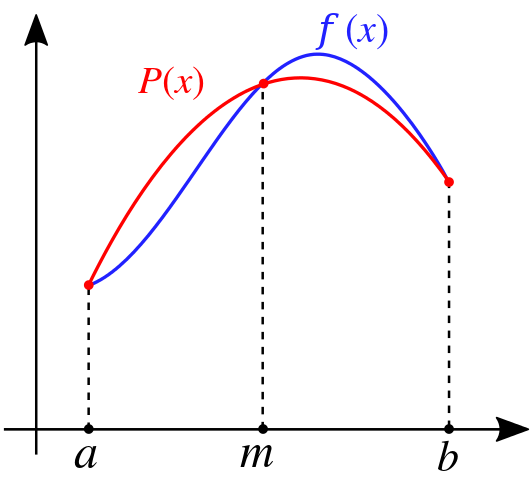
\includegraphics [scale=0.4] {simpson's_rule.png} \end{center}

We sample once each from $a$ and $b$, and four times from $m$, and average those samples.

The trapezoidal rule is
\[ \frac{f(a) + f(b) }{2} \cdot (b-a) \]
\begin{center} 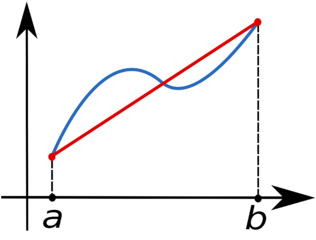
\includegraphics [scale=0.6] {trapezoidal_rule.png} \end{center}

Simpson's rule is really just a combination of the other two rules, namely, it is equal to $(2M + T) / 3$.  It weights the value at each endpoint as $1 \times$ and then the midpoint as twice the combined values at the endpoints.

Essentially, this fits a parabola to the points $a,m,b$ and then computes the area.  It is really Archimedes' result (quadrature) in disguise.

Consider the parabola $y = -x^2 + 1$ between $x=-1 \rightarrow 1$ (the points where it crosses the $x$-axis on its way down).  Our task is to find the correct $y$-value to use as the average height of the function in this region.  Inverting the standard result for the area under $y=x^2$, the area under this parabola is $2/3$ of the area above it.  The result we seek is $2/3$.

So a quadratic approximation to the area samples four times at the vertex plus once each at $x= \pm 1$.   We sample because we understand that the curve is probably not exactly quadratic.

\end{document}